\documentclass{amsart}
\usepackage[margin=3cm]{geometry}                % See geometry.pdf to learn the layout options. There are lots.
\geometry{letterpaper}                   % ... or a4paper or a5paper or ...
%\geometry{landscape}                % Activate for for rotated page geometry
\usepackage[parfill]{parskip}    % Activate to begin paragraphs with an empty line rather than an indent
\usepackage{float}
\usepackage{graphicx}
\usepackage{amssymb}
\usepackage{epstopdf}
\usepackage{siunitx}
\usepackage{subcaption}
\usepackage{listings}
\usepackage{setspace}
\usepackage{units}
\usepackage{amsmath}
\usepackage{wrapfig}
\usepackage{lscape}


\DeclareGraphicsRule{.tif}{png}{.png}{`convert #1 `dirname #1`/`basename #1 .tif`.png}
\graphicspath{{./img/}}

\title{Swinging Gate Pendulum Seismometer}
\author{Caspar \textsc{Lant}} % Author name

\date{\today} % Date for the report

\begin{document}

\bigskip

\maketitle % Insert the title, author and date
\begin{center}

Intermediate Experimental Physics II\\
\vspace{1.5cm}

\begin{tabular}{l r}

Section: & 002\\
\\
Date Performed: & February 16, 2016 \\ % Date the experiment was performed
Date Due: & February 23, 2016\\
\\
Partner: & Neil Saddeler\\ % Partner names
Professor: & Prof. Andrew Kent\\
Instructor: & David Mykytyn % Instructor/supervisor
\end{tabular}
\vfill
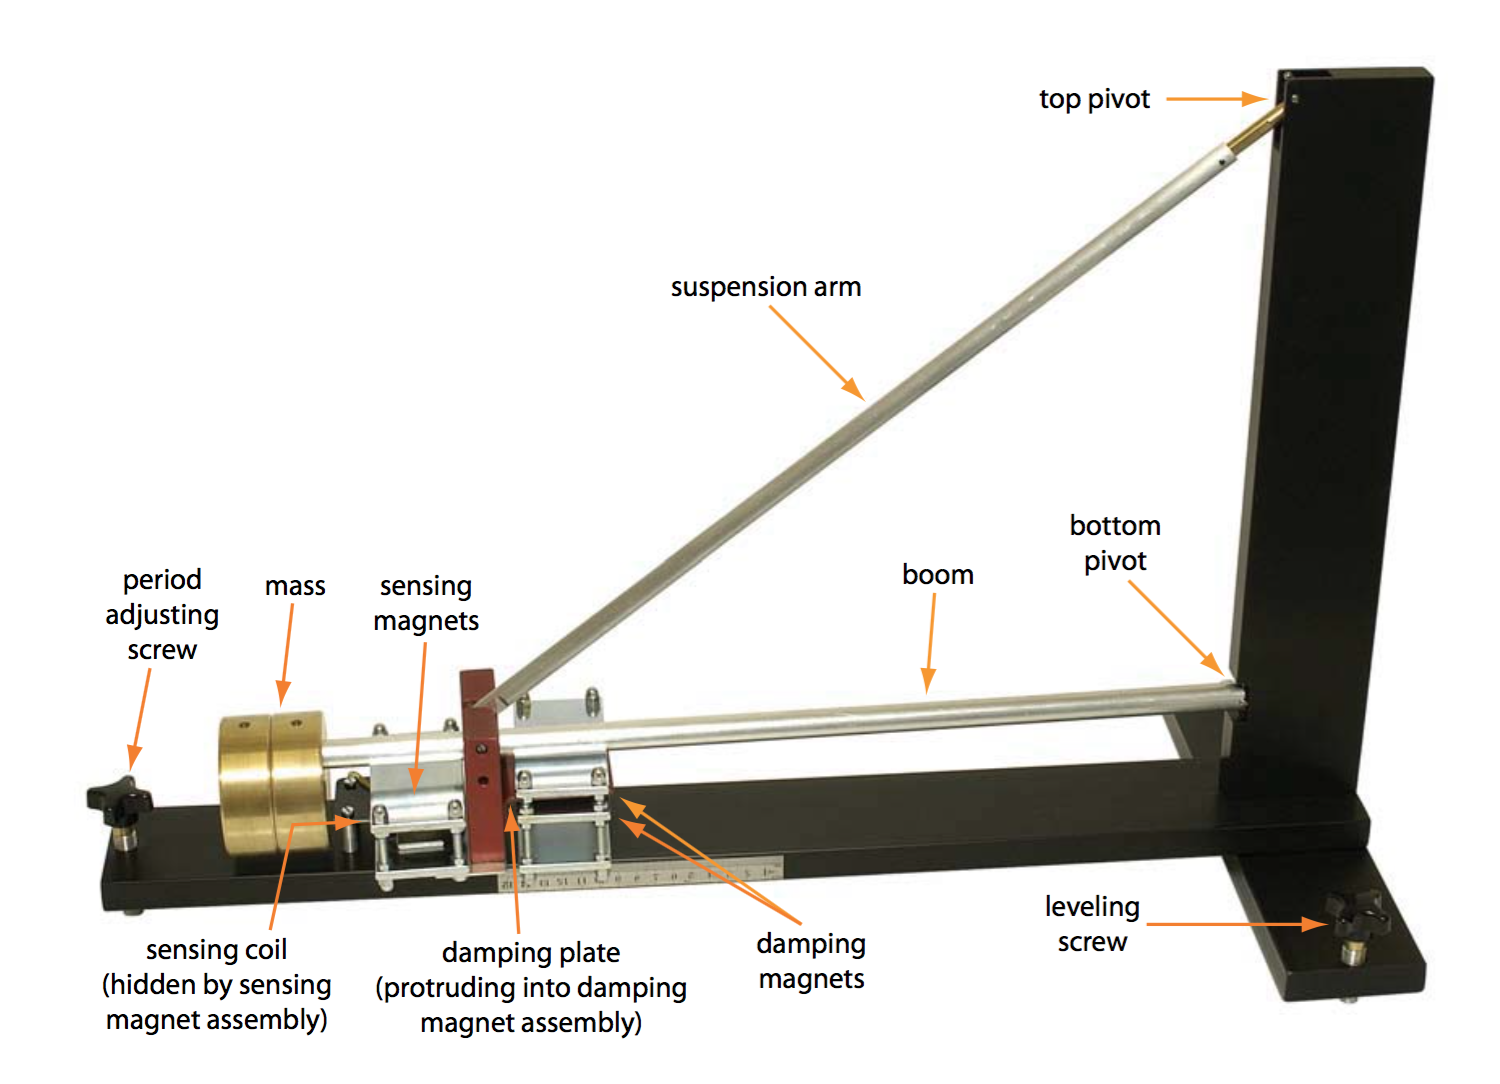
\includegraphics[width=0.7\textwidth]{seismo.png}
\vfill
\end{center}
\pagebreak
\setstretch{1.4}

\paragraph{\textbf{The Objective} of this week's experiment was to use an oscilloscope to futher our understanding of damping and driving effects in oscillitory systems.}

\section{Theoretical Background/ Abstract}
Seismometers are of interest because they allow us to detect otherwise unnoticed mechanical vibrations in the world arround us. This is very useful in the detection of earthquakes and all sorts of geologic phenomena. Careful analysis of data produced by precise seismometers can allow us to predict the severity of earthquakes well before they happen. It's important to note that, although mechanical waves propegate longitudinally in air (as sound), they are transversely-propegating in solids like the earth's mantel and crust. It is for this reason that seismometers detect the transverse movement of earth, which is to say up and down. The device used in this lab is a ``swinging gate" siesmometer, which is sensitive to vibrations on the order of tens of micrometers in amplitude.\\
In this lab we will measure the damping effects of a magnet placed under our seismometer, take measurements of the devices response to a driving oscillation, and take a noise measurement in which we will observe the passing of the N and R trains.
\vspace{5pt}
\begin{figure}[H]
    %
    \begin{minipage}{.255\textwidth}
        \vspace{-5pt}
        \centering
        \begin{equation*}
            \begin{split}
                0 &= m\ddot x + \Gamma \dot x + kx \\
                &\Rightarrow  \ddot x + \nicefrac{\Gamma}{m} \dot x + \nicefrac{k}{m} x \\
                &\Rightarrow  \ddot x + \gamma \dot x + \omega_0^2 x
            \end{split}
        \end{equation*}
    \end{minipage}
    %
    \begin{minipage}{.734\textwidth}
        \setstretch{1.4}
        The derivation of the general equation of motion for an underdamped vibration is given to the left. We expect the seismometer to be underdamped for most magnet positions, and that the damping constant will increase with increasing distance btween the magnet and the pendulum's pivot point.
    \end{minipage}
\end{figure}
\vspace{-15pt}
From the ODE above, and some educated-guessing, we come to the following value of $x(t)$:
\begin{equation}
    x_u(t) = \frac{1}{2} e^{\nicefrac{\gamma}{2}t}\left(a e^{i\omega_u t} + a^* e^{-i\omega_u t}\right)
\end{equation}
Where $\omega_u = \sqrt{\omega_0^2 - \left(\nicefrac{\gamma}{2}\right)^2} > 0$, and $a^*$ is $a$'s complex conjugate. The value of those two constants is given by initial systemic conditions\-- displacement, intial velocity, etc.

\section{Experimental Procedure}

\setstretch{1.3}
\begin{enumerate}
    \item Level the seismometer by adjusting the thumbscrew on its base. It turns out that the best way to do this is not with the provided bubble level, but by eye. You should  adjust the screw to a height such that the device's pendulum finds its equillibrium position at the middle of the seismometer base.
    \item Turn on data studio and set up a display of pendulum position versus time.
    \item Move the magnet to the non-business end of the device. Blow on the pendulum to displace it slightly.
    \item Measure the Period of the oscillations in DataStudio and dial in the second thumbscrew (located at the end of the pendulum's base) such that the period is between 14 adn 16 seconds.
    \item Once you're satisfied with your leveling, blow on the pendulum again and record about a dozen cycles. Note that if the pendulum's motion dies out before ten cycles, you should be blowing harder.
    \item Repeat this prodecure for various magnet positions. You should see an increasing damping effect.
    \item Export all this data for future analysis.
    \item Future analysis: pass each dataset into the provided python script and fit them curves! Record the values for amplitude, period, phase shift, and the damping factor.
    \item Next, Hook up the mechanical vibrator to DataStudio and pass a square wave through it at a relatively low frequency.
    \item Position the acrylic rod connected to the vibrator such that it comes into contact with the base of the seismometer.
    \item Measure the damping response for a sampling of frequencies.
    \item Remove the device from its inner tubes and repeat the last three steps.
    \item Now, turn off the vibrator and take a noise sample. Be on the lookout for peaks caused by passing trains.
    \item Export all this data as well. You're done.
\end{enumerate}
\section{Damping Effects}
\setstretch{1.4}

We predict that the damping coeffecient for our oscillitory system will increase as the distance bewteen the magnet and the pendulum mass decreases. This has to do with the fact that our pendulum seismometer can be thought of as a lever. When the force produced by the interaction between the magnet and the pendulum is closest to the end of the pendulum, it produces the greatest torque, and has the greatest mechanical advantage. \\ \\
\setstretch{1.3}
Figure 1 tracks the oscillation of our measurement device with the magnet removed. The damping effects seen are produced by frictional forces and air resitance.\\ \\
Figure 2 shows the movement of our pendulum with the magnet $\unit[5]{cm}$ from our zero point. It is fitted with a time-damped sine curve.\\ \\
Figure 3 plots the oscillation of the seismometer for three magnet positions. The overdamped case is shown in red.\\ \\
Figure 4 shows the micro oscillations present in the overdamped case, and a fit-cure. The parameters of the fit are displayed in the upper-righthand corner of the graph.
\setcounter{figure}{4}
\section{Noise Sample - Locomotion Commotion}
\setcounter{page}{4}

\setstretch{1.4}

Although Neil, with his head against the table, was able to hear trains pass, the trains did not produce an amplitude on the seismometer that exceeded our noise threshold. My guess is that, given that the seismometer is more sensitive to amplitude than Neil's ears are, Neil was able to detect the passing of a train not because of an elevated amplitude, but because of the characteristic vibratory envelope of a train passing. You'll see that the peaks labled ``train" are each bordered by a ``ramp-up" on its left and a ``ramp-down" in amplitude on its right. This is consistant with our intuition surrounding passing trains. My first impulse was to compare our data to MTA train schedules, but it soon became clear that the discrepencies between scheduled and actual train arrival times was often larger than the frequency at which train arrivals occur! This is to say that MTA train schedules are totally useless, or at least only good for providing an idea of the frequency of trains at a given time of day. If we were to design ``train seismometer"\-- one who's sole purpose was to record vibratory signature of passing trains, our first move would be to place the device as close to the source of vibration as possible, and also to taylor the resonant frequency of the device to match the vibrating frequency of our test-subjects. I'd probably hire an acousician to do this for me. It's also important to note that the only trains that are marked on this graph are those which passed through the station without stopping\-- known as ``express" trains. Local trains, which stopped in our local station, have slowed down so much by the time that they reach us that the amplitude of the vibrations that they produce is negligible. You'll notice that on of the largest peaks in amplitude occurs towards the very beginning of our sample span. This is likely an artifact of my setting up the device; pehaps a footstep I placed as I settled back into my chair from DataStudio...
% \vspace{-0.1cm}
\begin{figure}[H]
    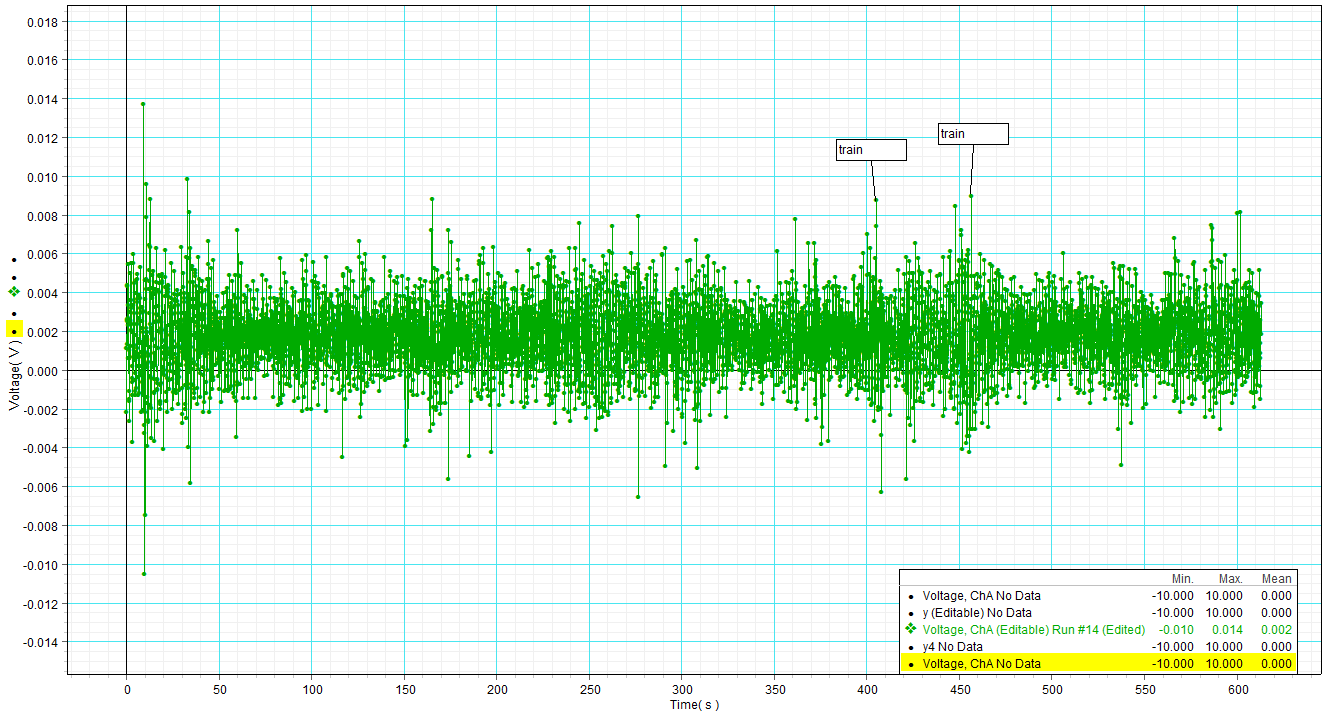
\includegraphics[width=0.95\textwidth]{train2.png}
    \caption{Noise Sample with Train Markers}
\end{figure}

\section{Driven Oscillations}
Figure \ref{fig:interference} shows the seismometer's response to a mechanical oscillation with frequency of $\unit[10]{Hz}$. The dark inner bands are an interference pattern produced by the interaction between the driving oscillation and the seismometer's sympathetic resonance. I would guess that the periodicity of this interference pattern is related to the natural resonant frequency of the measurement device.
\vfill
\begin{figure}[h]
    \centering
    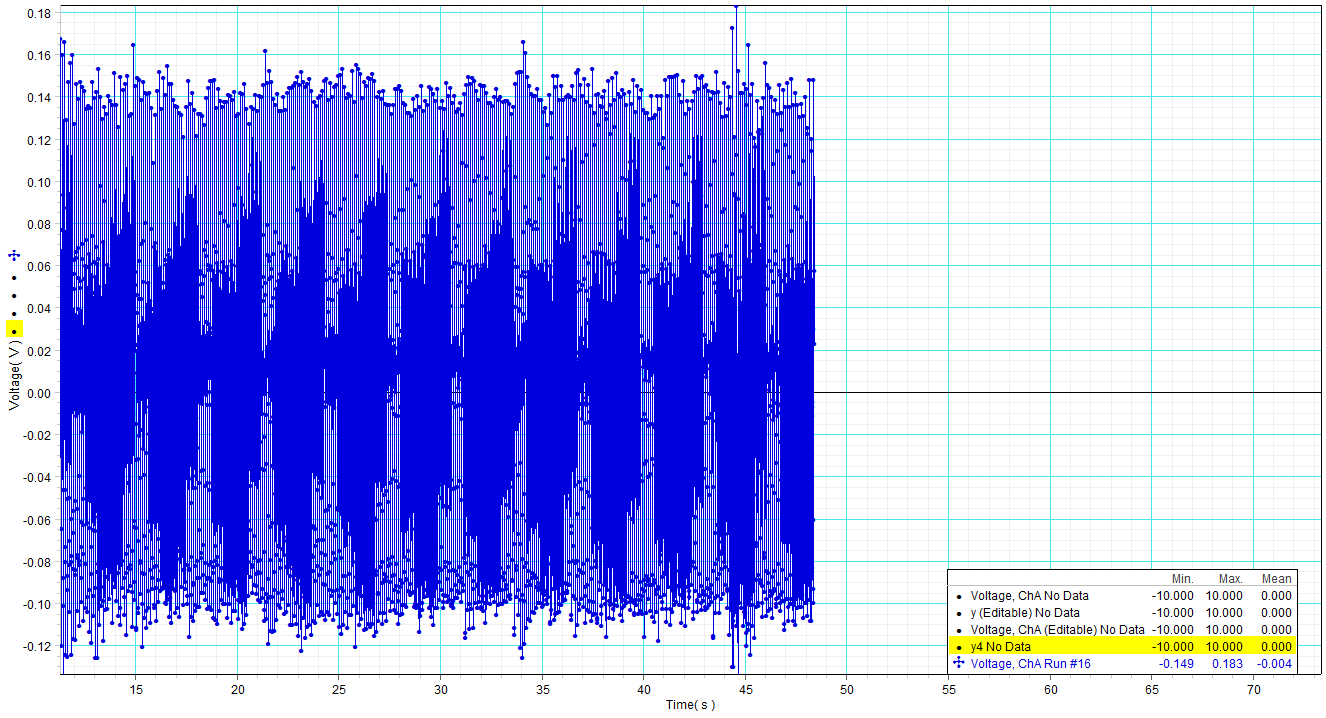
\includegraphics[width=0.95\textwidth]{vib1.png}
    \caption{Seismometer Response to $\unit[10]{Hz}$ Vibratory Disturbance}
    \label{fig:interference}
\end{figure}
\begin{figure}[H]
    \centering
    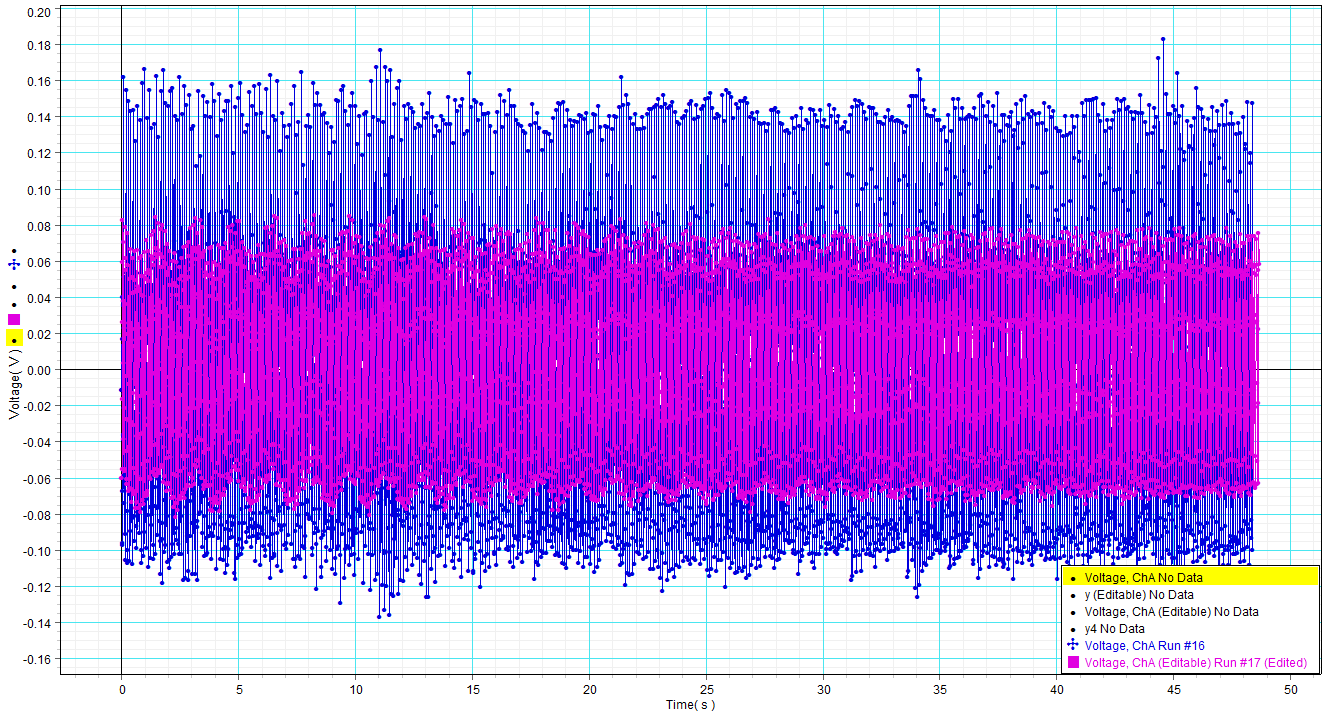
\includegraphics[width=0.95\textwidth]{vib2.png}
    \caption{Driven Oscillation with and without Vibration Isolation}
    \label{fig:vibrationisolation}
\end{figure}
\setstretch{1.4}
\section{Questions}

\textit{Repeat your measurements both with and without the vibration isolation mounts for the wooden table. Do you see a difference? Why or why not?}
\begin{quote}
    The amplitude of the noise increases by a factor of two when the vibration isolation mounts (inner tubes) are removed. It's also clear that the seismometer was no leveled correctly when taken off its inner tubes\-- the noise graph with larger amplitude centers itself around a voltage not equal to zero. See Figure \ref{fig:vibrationisolation}.
\end{quote}


\section{Error Analysis}
In this experiment, our greatest source of error was certainly the erranous vibratory disturbances present in a laboratory full of people conducting their own experiments, oblivious to the fact that a pair of their classmates were taking mesaurements from an extremely precise instrument, and were acutely aware of their footstep. This could be mitigated by increasing the efficacy of the vibration oscillation mounts, perhaps by inflating them less, or by kicking everyone else out of the classroom. Another frustration was the fact that the pendulum on the seismometer refused to be centered. This produced a slight vertical offset in our noise measurements as well as an additional layer of uncertainty in our measurement of damping effects. This could be recitfied by a more precise instrument, and with more time spent calibrating it. Judging on our few measurements for magnet placement, I'd say that the damping factor is exponentially dependent on the distance between the magnet and the pivot point of the oscilloscope. I figure this because there is a relatively small difference in quality factor between magnet positions one two and three but a rather large one between positions three and four. Not the best analysis of this, but it's consistent with my understanding of torque and damped oscillitory systems, so I'd say that it's enough to go on...
\vspace{0.2cm}
\begin{figure}[H]
    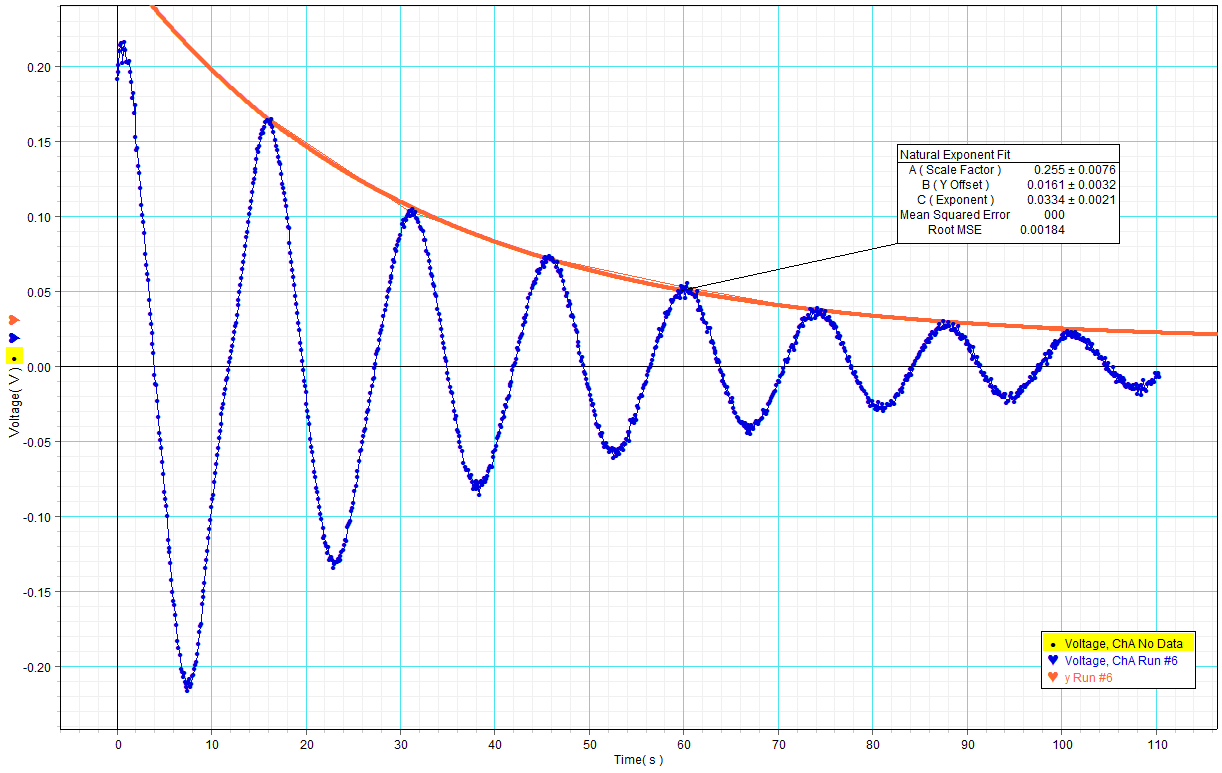
\includegraphics[width=0.7\textwidth]{dampedwithfit.png}
\end{figure}

\newpage
\setstretch{1.2}
\lstinputlisting[language=Python]{./data/ReadDataFitPlot.py}

\end{document}
